\documentclass{beamer}

\usepackage{polyglossia}

\usepackage[orientation = portrait, size = a1, scale = 1.4]{beamerposter}
\usepackage[backend = biber, style = iso-authoryear, sortlocale = en_US, autolang = other, bibencoding = UTF8]{biblatex}
\usepackage{datetime}
\usepackage{adjustbox}
%\usepackage[utf8]{inputenc}
\usepackage{fontspec}
\usepackage{mathrsfs}
\usepackage{microtype}
\usepackage{listings}
\usepackage{booktabs}

\setdefaultlanguage{english}
\setmainfont{TeX Gyre Termes}
\usetheme{gemini}
\usecolortheme{mit}

\usepackage{tikz}
\usepackage{pgfplots}
\usetikzlibrary{arrows,automata,shapes,calc, patterns, backgrounds}
\input{images/tikzlib}

\definecolor{gray}{rgb}{0.5,0.5,0.5}
\definecolor{mauve}{rgb}{0.58,0,0.82}
\lstset{basicstyle={\small\ttfamily},
	belowskip=3mm,
	breakatwhitespace=true,
	breaklines=true,
	classoffset=0,
	columns=flexible,
	framexleftmargin=0.25em,
	frameshape={}{}{}{}, %To remove to vertical lines on left, set `frameshape={}{}{}{}`
	keywordstyle=\color{blue},
	numbers=none, %If you want line numbers, set `numbers=left`
	numberstyle=\color{gray},
	showstringspaces=false,
	stringstyle=\color{mauve},
	tabsize=3,
	xleftmargin =1em
}

\DeclareMathOperator*{\argmax}{arg\,max}
\def\mathdefault#1{#1}

\title{Representation learning for structured data}

\author{%
	Marek Dědič\inst{1 2}
}
\institute{%
	\inst{1} Czech Technical University in Prague \samelineand
	\inst{2} Cisco Systems, Inc.
}

\footercontent{%
	DC @ ECAI 2025, Bologna, Italy \hfill
	\href{mailto:marek@dedic.eu}{marek@dedic.eu}
}

% \logoright{\includegraphics[height=7cm]{logo1.pdf}}
% \logoleft{\includegraphics[height=7cm]{logo2.pdf}}

% If you have N columns, choose \sepwidth and \colwidth such that
% (N+1)*\sepwidth + N*\colwidth = \paperwidth
\newlength{\sepwidth}
\newlength{\colwidth}
\setlength{\sepwidth}{0.033\paperwidth}
\setlength{\colwidth}{0.45\paperwidth}
\newcommand{\separatorcolumn}{\begin{column}{\sepwidth}\end{column}}

\newcommand{\corr}{(\Letter)}
\newcommand{\name}[1]{\textit{#1}}
\newcommand{\mathfield}{\ensuremath{\mathbb}}
\newcommand{\mathmat}{\ensuremath{\mathbf}}
\newcommand{\mathset}{\ensuremath{\mathbb}}
\newcommand{\mathspace}{\ensuremath{\mathcal}}
\newcommand{\mathvec}{\ensuremath{\bm}}

\newcommand{\method}{CSP}
\newcommand{\methodlong}{Convolutional Signal Propagation}
\newcommand{\U}{V} % set of nodes in hypergraph
\newcommand{\uu}{v} % node in hypergraph
\newcommand{\V}{E} % set of hyperedges in hypergraph
\newcommand{\vv}{e} % hyperedge in hypergraph
\newcommand{\HG}{\mathcal{H}} % hypergraph
\newcommand{\HH}{\mathmat{H}} % incidence matrix
\newcommand{\BG}{\mathcal{G}_\mathrm{bip}} % bipartite graph
\newcommand{\E}{E_\mathrm{bip}} % set of edges in bipartite graph
\newcommand{\D}{\mathmat{D}_v} % node degree matrix
\newcommand{\B}{\mathmat{D}_e} % hyperedge degree matrix
\newcommand{\X}{\mathmat{X}} % feature matrix
\newcommand{\Y}{\mathmat{Y}} % label matrix
\newcommand{\y}{y} % label
\newcommand{\x}{\mathvec{x}} % feature vector
\newcommand{\Tr}{V_\mathrm{train}} % Training set
\newcommand{\vdeg}{\mathrm{d}} % degree of node or edge
\newcommand{\edeg}{\delta} % degree of node or edge

\begin{document}
\begin{frame}[fragile,t]

\begin{columns}[t]
	\separatorcolumn

	\begin{column}{\colwidth}
		\begin{block}{The performance-complexity trade-off}
			Graph neural networks (GNNs) suffer from high computational demands, which may be a prohibitive issue in some applications. We investigate the interplay of graph coarsening and the performance of a downstream task. The main aim of this work is to explore the performance-complexity characteristics in the context of graph learning.
			\begin{figure}
				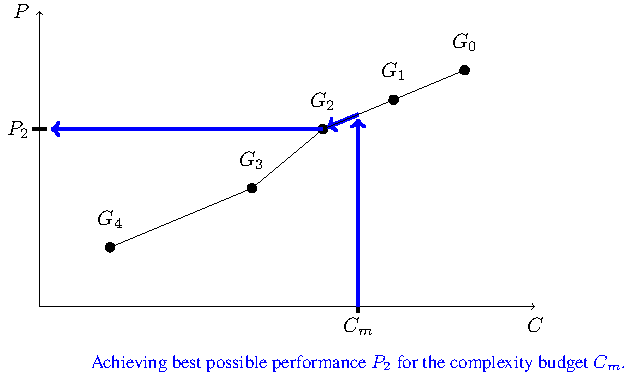
\includegraphics[width=0.8\linewidth]{images/performance-complexity/performance-complexity.pdf}
			\end{figure}
		\end{block}

		\begin{block}{HARP pipeline overview}
			Our work builds on the HARP method for pretraining on coarsened graphs.
			\begin{figure}
				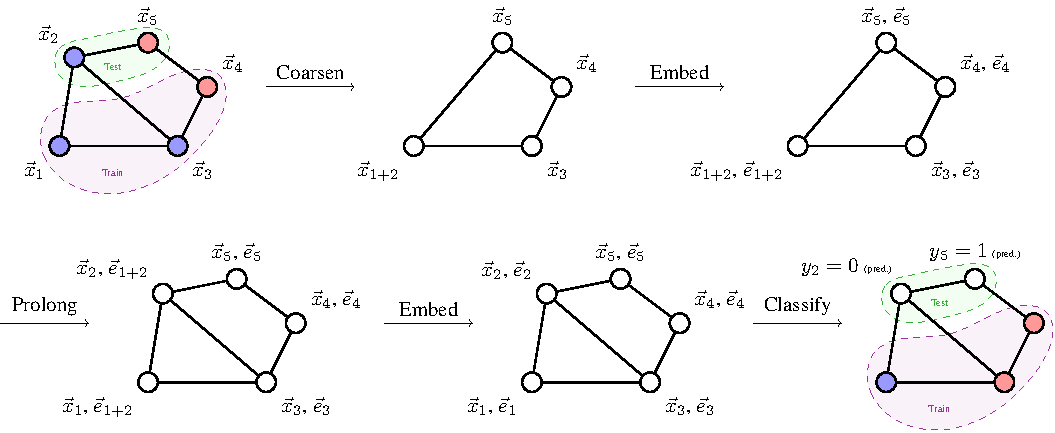
\includegraphics[width=\linewidth]{images/harp-overview/harp-overview.pdf}
			\end{figure}
		\end{block}

		\begin{block}{Adaptive prolongation}
			The main contribution of this work is the adaptive prolongation schema. The algorithm works with the pre-coarsened graphs produced by HARP, however, the prolongation steps are decoupled from the coarsening steps.
			\begin{figure}
				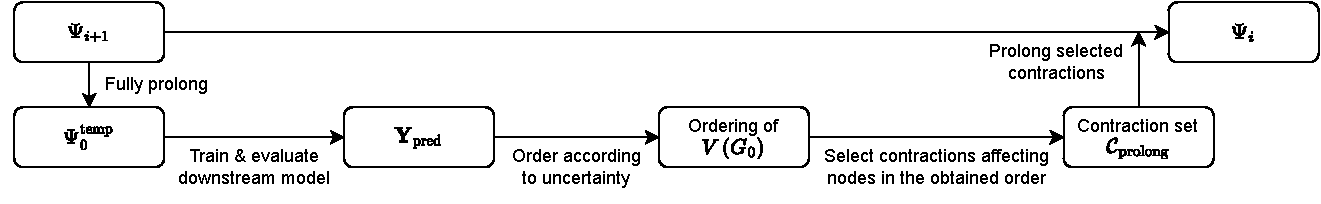
\includegraphics[width=\linewidth]{images/adaptive-prolongation/adaptive-prolongation.pdf}
			\end{figure}
		\end{block}

		\begin{block}{Results}
			\begin{figure}
				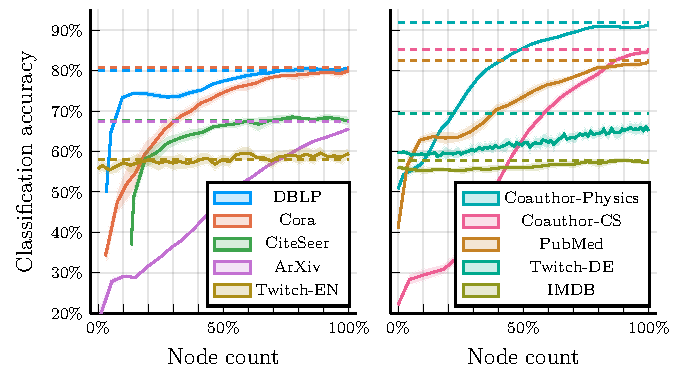
\includegraphics[width = 0.95\linewidth]{images/adaptive-coarsening/adaptive-coarsening.pdf}
			\end{figure}
		\end{block}
	\end{column}

	\separatorcolumn

	\begin{column}{\colwidth}
		\begin{alertblock}{3 main projects}
			\begin{itemize}
				\item A HARP-based method for solving performance-complexity trade-off in GNNs via adaptive prolongation.
				\item CSP is a very simple learning method for classification and retrieval on graphs, hyper-graphs or problems described by one-hot features. It achieves comparable performance to reference methods in multiple problems, while being significantly cheaper to compute.
			\end{itemize}
		\end{alertblock}

		\begin{block}{Convolutional Signal Propagation (CSP)}
			\begin{center}
				\adjustbox{width=0.8\columnwidth}{%
					\begin{tikzpicture}
\tikzset{node/.style={draw,circle}}
\tikzset{edge/.style={draw,rectangle,inner sep=2pt}}

\tikzset{nodepos/.style={draw,circle, fill=red!20!white}}
\tikzset{nodestress/.style={draw,circle, ultra thick}}




%% Bipartite Graph
\begin{scope}[node distance=2.4cm, circle, draw=black]
    \node[nodepos] at (0, -2) (x1) {$\uu_1$};
    \node[nodepos, below of=x1] (x2) {$\uu_2$};
    \node[nodestress, below of=x2] (x3) {$\uu_3$};
    \node[node, below of=x3] (x4) {$\uu_4$};
    \node[node, below of=x4] (x5) {$\uu_5$};
\end{scope}
    
\begin{scope}[node distance=3.2cm]
    \node[node] at (4, -2) (e1) {$\vv_1$};
    \node[node, below of=e1] (e2) {$\vv_2$};
    \node[node, below of=e2] (e3) {$\vv_3$};
    \node[node, below of=e3] (e4) {$\vv_4$};
\end{scope}

  \draw (e1) -- (x3);
  \draw (e1) -- (x1);
  \draw (e1) -- (x2);
  \draw (e2) -- (x2);
  \draw (e2) -- (x1);
  \draw (e4) -- (x1);
  \draw (e1) -- (x5);
  \draw (e2) -- (x4);
  \draw (e4) -- (x3);
  \draw (e3) -- (x4);
  \draw (e3) -- (x5);


    






%% Hyper-Graph

\begin{scope}[xshift=11cm, yshift=-7cm]
    \node[nodepos] at (0:4) (xx2) {$\uu_2$};
    \node[nodepos] at (72:4)(xx1) {$\uu_1$};
    \node[nodestress] at (144:4)(xx3) {$\uu_3$};
    \node[node] at (216:4)(xx5) {$\uu_5$};
    \node[node] at (288:4)(xx4) {$\uu_4$};

\end{scope}

  %\draw (ee1) -- (xx3);
  %\draw (ee1) -- (xx1);
  %\draw (ee1) -- (xx2);
  %\draw (ee2) -- (xx2);
  %\draw (ee2) -- (xx1);
  %\draw (ee4) -- (xx1);
  %\draw (ee1) -- (xx5);
  %\draw (ee2) -- (xx4);
  %\draw (ee4) -- (xx3);
  %\draw (ee3) -- (xx4);
  %\draw (ee3) -- (xx5);

\begin{scope}[fill opacity=0.2]
    \filldraw[fill=yellow!20] ($(xx1)+(1,0)$) 
        to[out=90,in=0] ($(xx1) + (0,1)$) 
        to[out=180,in=70] ($(xx3) + (-1,0)$) 
        to[out=250,in=210] ($(xx3) + (0,-1)$)
        to[out=30,in=270] ($(xx1) + (1,0)$);
    \filldraw[fill=green!20] ($(xx5)+(-1,0)$) 
        to[out=250,in=180] ($(xx5) + (0,-1)$) 
        to[out=0,in=210] ($(xx4) + (0,-1)$) 
        to[out=30,in=290] ($(xx4) + (1, 0)$)
        to[out=110,in=70] ($(xx5) + (-1,0)$);
    \filldraw[fill=cyan!20] ($(xx1)+(-1,0)$) 
        to[out=270,in=90] ($(xx4) + (-1,0)$) 
        to[out=270,in=180] ($(xx4) + (0,-1)$) 
        to[out=0,in=270] ($(xx2) + (1,0)$) 
        to[out=90,in=0] ($(xx1) + (0, 1)$)
        to[out=180,in=90] ($(xx1) + (-1, 0)$);
    \filldraw[fill=gray!20] ($(xx1)+(0,1)$) 
        to[out=180,in=90] ($(xx3) + (-1,0)$) 
        to[out=270,in=210] ($(xx5) + (0,-1)$) 
        to[out=30,in=270] ($(xx2) + (1,0)$) 
        to[out=90,in=0] ($(xx1) + (0, 1)$);
\end{scope}


\begin{scope}[xshift=20cm, yshift=-3cm]
\node at (0,0) {%
    $\mathmat{H}=\left[\begin{array}{cccc}
 1 & 1 & 0 & 1 \\
 1 & 1 & 0 & 0 \\
 1 & 0 & 0 & 1 \\
 0 & 1 & 1 & 0 \\
 1 & 0 & 1 & 0 
     \end{array}
     \right]$
};

\end{scope}

\begin{scope}[xshift=20cm, yshift=-9cm]
\node at (0,0) {%
     $\mathmat{Y}=\left[\begin{array}{c}
 1 \\
 1 \\
 0 \\
 0 \\
 0 
     \end{array}
     \right]$
};

\end{scope}

\end{tikzpicture}

				}
			\end{center}
			\begin{equation*}
				\hspace*{-1.5cm}
				x_k^{(l+1)} = \underbrace{%
					\frac{1}{deg\left( \uu_k \right)}\sum_{\substack{j \\ \uu_k \in \vv_j}}
				}_{\mathrm{2nd~step}} \
				\underbrace{
					\frac{1}{deg \left( \vv_j \right)}\sum_{\substack{i \\ \uu_i \in \vv_j}} x_i^{(l)}
				}_{\mathrm{1st~step}},\quad
				\mathmat{X}^{(l+1)} = \underbrace{\D^{-1} \HH}_{\mathrm{2nd~step}} \ \underbrace{\B^{-1} \HH^T \mathmat{X}^{(l)}}_{\mathrm{1st~step}}
			\end{equation*}
		\end{block}

		\begin{block}{CSP Retrieval Results -- P@{}100, exectution time in \(\mu s \)}
			\adjustbox{width=\columnwidth}{%
				\begin{tabular}{lrrrrrrrr}
					\textbf{Method} & \textbf{CiteSeer} & \textbf{Cora-CA} & \textbf{Cora-CC} & \textbf{DBLP} & \textbf{PubMed} & \textbf{Corona} &\textbf{movie-RA} & \textbf{movie-TA} \\
					\midrule
					\textbf{\method{} 1-layer} & 0.494 & \underline{0.703} & 0.530 & 0.869 & 0.798 & \textbf{0.530} & 0.334 & 0.156 \\
					\textbf{\method{} 2-layer} & \underline{0.558} & \underline{0.718} & \underline{0.681} & 0.865 & \underline{0.826} & 0.440 & 0.336 & 0.186 \\
					\textbf{\method{} 3-layer} & \textbf{0.568} & \textbf{0.721} & \textbf{0.707} & 0.869 & \underline{0.850} & 0.332 & 0.238 & 0.186 \\
					\textbf{Naive Bayes} & 0.471 & \underline{0.686} & 0.491 & \textbf{0.951} & \underline{0.860} & 0.446 & 0.216 & 0.153 \\
					\textbf{HGCN-NMF} & 0.482 & \underline{0.671} & 0.607 & 0.794 & \textbf{0.871} & 0.392 & 0.257 & 0.148 \\
					\textbf{LR-NMF} & 0.329 & 0.603 & 0.372 & 0.602 & 0.735 & 0.397 & \textbf{0.580} & \textbf{0.356} \\
					\textbf{RF-NMF} & 0.303 & 0.474 & 0.482 & 0.843 & 0.794 & 0.381 & 0.470 & 0.131 \\
					\textbf{Random} & 0.153 & 0.132 & 0.129 & 0.155 & 0.308 & 0.180 & 0.040 & 0.055 \\
					\bottomrule
				\end{tabular}
			}

			\adjustbox{width=\columnwidth}{%
				\begin{tabular}{lrrrrrrrr}
					\textbf{Method} & \textbf{CiteSeer} & \textbf{Cora-CA} & \textbf{Cora-CC} & \textbf{DBLP} & \textbf{PubMed} & \textbf{Corona} & \textbf{movie-RA} & \textbf{movie-TA} \\
					\midrule
					\textbf{\method{} 1-layer} & \textbf{1.35} & \textbf{1.23} & \textbf{1.24} & \textbf{3.51} & \textbf{4.01} & \textbf{22.83} & 170.63 & \textbf{12.07} \\
					\textbf{\method{} 2-layer} & 2.41 & 2.25 & 2.24 & 7.46 & 7.35 & 47.39 & 349.67 & 25.88 \\
					\textbf{\method{} 3-layer} & 3.31 & 3.09 & 3.08 & 9.65 & 9.1 & 70.98 & 506.1 & 35.75 \\
					\textbf{Naive Bayes} & 2.59 & 2.73 & 2.54 & 11.16 & 5.35 & 89.3 & 1 051.53 & 35.61 \\
					\textbf{*HGCN-NMF} & 23 714 & 23 690 & 23 709 & 29 123 & 23 879 & 112 314 & 620 717 & 70 778 \\
					\textbf{*LR-NMF} & 44.45 & 51.59 & 49.54 & 64.96 & 44.69 & 56 & \textbf{61.82} & 74.07 \\
					\textbf{*RF-NMF} & 140.76 & 143.85 & 134.52 & 1 148.83 & 323.6 & 1 608.58 & 697.85 & 716.68 \\
					\bottomrule
				\end{tabular}
			}
		\end{block}

		\begin{block}{Hyperparameter optimization for GNNs}
			We benchmarked 5 standard HPO methods on 9 GNN datasets. The results show that Bayesian optimization (BO) and Tree-structured Parzen Estimators (TPE) achieve the best performance, while Quasi Monte-Carlo (QMC) falls behind.
			\adjustbox{width=\columnwidth}{%
				%% Creator: Matplotlib, PGF backend
%%
%% To include the figure in your LaTeX document, write
%%   \input{<filename>.pgf}
%%
%% Make sure the required packages are loaded in your preamble
%%   \usepackage{pgf}
%%
%% Also ensure that all the required font packages are loaded; for instance,
%% the lmodern package is sometimes necessary when using math font.
%%   \usepackage{lmodern}
%%
%% Figures using additional raster images can only be included by \input if
%% they are in the same directory as the main LaTeX file. For loading figures
%% from other directories you can use the `import` package
%%   \usepackage{import}
%%
%% and then include the figures with
%%   \import{<path to file>}{<filename>.pgf}
%%
%% Matplotlib used the following preamble
%%   \def\mathdefault#1{#1}
%%   \everymath=\expandafter{\the\everymath\displaystyle}
%%   \IfFileExists{scrextend.sty}{
%%     \usepackage[fontsize=12.000000pt]{scrextend}
%%   }{
%%     \renewcommand{\normalsize}{\fontsize{12.000000}{14.400000}\selectfont}
%%     \normalsize
%%   }
%%   
%%   \makeatletter\@ifpackageloaded{underscore}{}{\usepackage[strings]{underscore}}\makeatother
%%
\begingroup%
\makeatletter%
\begin{pgfpicture}%
\pgfpathrectangle{\pgfpointorigin}{\pgfqpoint{8.000000in}{4.000000in}}%
\pgfusepath{use as bounding box, clip}%
\begin{pgfscope}%
\pgfsetbuttcap%
\pgfsetmiterjoin%
\definecolor{currentfill}{rgb}{1.000000,1.000000,1.000000}%
\pgfsetfillcolor{currentfill}%
\pgfsetlinewidth{0.000000pt}%
\definecolor{currentstroke}{rgb}{1.000000,1.000000,1.000000}%
\pgfsetstrokecolor{currentstroke}%
\pgfsetdash{}{0pt}%
\pgfpathmoveto{\pgfqpoint{0.000000in}{0.000000in}}%
\pgfpathlineto{\pgfqpoint{8.000000in}{0.000000in}}%
\pgfpathlineto{\pgfqpoint{8.000000in}{4.000000in}}%
\pgfpathlineto{\pgfqpoint{0.000000in}{4.000000in}}%
\pgfpathlineto{\pgfqpoint{0.000000in}{0.000000in}}%
\pgfpathclose%
\pgfusepath{fill}%
\end{pgfscope}%
\begin{pgfscope}%
\pgfsetbuttcap%
\pgfsetmiterjoin%
\definecolor{currentfill}{rgb}{1.000000,1.000000,1.000000}%
\pgfsetfillcolor{currentfill}%
\pgfsetlinewidth{0.000000pt}%
\definecolor{currentstroke}{rgb}{0.000000,0.000000,0.000000}%
\pgfsetstrokecolor{currentstroke}%
\pgfsetstrokeopacity{0.000000}%
\pgfsetdash{}{0pt}%
\pgfpathmoveto{\pgfqpoint{0.728496in}{0.650833in}}%
\pgfpathlineto{\pgfqpoint{7.820000in}{0.650833in}}%
\pgfpathlineto{\pgfqpoint{7.820000in}{3.820000in}}%
\pgfpathlineto{\pgfqpoint{0.728496in}{3.820000in}}%
\pgfpathlineto{\pgfqpoint{0.728496in}{0.650833in}}%
\pgfpathclose%
\pgfusepath{fill}%
\end{pgfscope}%
\begin{pgfscope}%
\pgfpathrectangle{\pgfqpoint{0.728496in}{0.650833in}}{\pgfqpoint{7.091504in}{3.169167in}}%
\pgfusepath{clip}%
\pgfsetroundcap%
\pgfsetroundjoin%
\pgfsetlinewidth{1.003750pt}%
\definecolor{currentstroke}{rgb}{0.800000,0.800000,0.800000}%
\pgfsetstrokecolor{currentstroke}%
\pgfsetdash{}{0pt}%
\pgfpathmoveto{\pgfqpoint{1.050837in}{0.650833in}}%
\pgfpathlineto{\pgfqpoint{1.050837in}{3.820000in}}%
\pgfusepath{stroke}%
\end{pgfscope}%
\begin{pgfscope}%
\definecolor{textcolor}{rgb}{0.150000,0.150000,0.150000}%
\pgfsetstrokecolor{textcolor}%
\pgfsetfillcolor{textcolor}%
\pgftext[x=1.050837in,y=0.518888in,,top]{\color{textcolor}{\sffamily\fontsize{11.000000}{13.200000}\selectfont\catcode`\^=\active\def^{\ifmmode\sp\else\^{}\fi}\catcode`\%=\active\def%{\%}$\mathdefault{0}$}}%
\end{pgfscope}%
\begin{pgfscope}%
\pgfpathrectangle{\pgfqpoint{0.728496in}{0.650833in}}{\pgfqpoint{7.091504in}{3.169167in}}%
\pgfusepath{clip}%
\pgfsetroundcap%
\pgfsetroundjoin%
\pgfsetlinewidth{1.003750pt}%
\definecolor{currentstroke}{rgb}{0.800000,0.800000,0.800000}%
\pgfsetstrokecolor{currentstroke}%
\pgfsetdash{}{0pt}%
\pgfpathmoveto{\pgfqpoint{2.027628in}{0.650833in}}%
\pgfpathlineto{\pgfqpoint{2.027628in}{3.820000in}}%
\pgfusepath{stroke}%
\end{pgfscope}%
\begin{pgfscope}%
\definecolor{textcolor}{rgb}{0.150000,0.150000,0.150000}%
\pgfsetstrokecolor{textcolor}%
\pgfsetfillcolor{textcolor}%
\pgftext[x=2.027628in,y=0.518888in,,top]{\color{textcolor}{\sffamily\fontsize{11.000000}{13.200000}\selectfont\catcode`\^=\active\def^{\ifmmode\sp\else\^{}\fi}\catcode`\%=\active\def%{\%}$\mathdefault{10}$}}%
\end{pgfscope}%
\begin{pgfscope}%
\pgfpathrectangle{\pgfqpoint{0.728496in}{0.650833in}}{\pgfqpoint{7.091504in}{3.169167in}}%
\pgfusepath{clip}%
\pgfsetroundcap%
\pgfsetroundjoin%
\pgfsetlinewidth{1.003750pt}%
\definecolor{currentstroke}{rgb}{0.800000,0.800000,0.800000}%
\pgfsetstrokecolor{currentstroke}%
\pgfsetdash{}{0pt}%
\pgfpathmoveto{\pgfqpoint{3.004419in}{0.650833in}}%
\pgfpathlineto{\pgfqpoint{3.004419in}{3.820000in}}%
\pgfusepath{stroke}%
\end{pgfscope}%
\begin{pgfscope}%
\definecolor{textcolor}{rgb}{0.150000,0.150000,0.150000}%
\pgfsetstrokecolor{textcolor}%
\pgfsetfillcolor{textcolor}%
\pgftext[x=3.004419in,y=0.518888in,,top]{\color{textcolor}{\sffamily\fontsize{11.000000}{13.200000}\selectfont\catcode`\^=\active\def^{\ifmmode\sp\else\^{}\fi}\catcode`\%=\active\def%{\%}$\mathdefault{20}$}}%
\end{pgfscope}%
\begin{pgfscope}%
\pgfpathrectangle{\pgfqpoint{0.728496in}{0.650833in}}{\pgfqpoint{7.091504in}{3.169167in}}%
\pgfusepath{clip}%
\pgfsetroundcap%
\pgfsetroundjoin%
\pgfsetlinewidth{1.003750pt}%
\definecolor{currentstroke}{rgb}{0.800000,0.800000,0.800000}%
\pgfsetstrokecolor{currentstroke}%
\pgfsetdash{}{0pt}%
\pgfpathmoveto{\pgfqpoint{3.981210in}{0.650833in}}%
\pgfpathlineto{\pgfqpoint{3.981210in}{3.820000in}}%
\pgfusepath{stroke}%
\end{pgfscope}%
\begin{pgfscope}%
\definecolor{textcolor}{rgb}{0.150000,0.150000,0.150000}%
\pgfsetstrokecolor{textcolor}%
\pgfsetfillcolor{textcolor}%
\pgftext[x=3.981210in,y=0.518888in,,top]{\color{textcolor}{\sffamily\fontsize{11.000000}{13.200000}\selectfont\catcode`\^=\active\def^{\ifmmode\sp\else\^{}\fi}\catcode`\%=\active\def%{\%}$\mathdefault{30}$}}%
\end{pgfscope}%
\begin{pgfscope}%
\pgfpathrectangle{\pgfqpoint{0.728496in}{0.650833in}}{\pgfqpoint{7.091504in}{3.169167in}}%
\pgfusepath{clip}%
\pgfsetroundcap%
\pgfsetroundjoin%
\pgfsetlinewidth{1.003750pt}%
\definecolor{currentstroke}{rgb}{0.800000,0.800000,0.800000}%
\pgfsetstrokecolor{currentstroke}%
\pgfsetdash{}{0pt}%
\pgfpathmoveto{\pgfqpoint{4.958002in}{0.650833in}}%
\pgfpathlineto{\pgfqpoint{4.958002in}{3.820000in}}%
\pgfusepath{stroke}%
\end{pgfscope}%
\begin{pgfscope}%
\definecolor{textcolor}{rgb}{0.150000,0.150000,0.150000}%
\pgfsetstrokecolor{textcolor}%
\pgfsetfillcolor{textcolor}%
\pgftext[x=4.958002in,y=0.518888in,,top]{\color{textcolor}{\sffamily\fontsize{11.000000}{13.200000}\selectfont\catcode`\^=\active\def^{\ifmmode\sp\else\^{}\fi}\catcode`\%=\active\def%{\%}$\mathdefault{40}$}}%
\end{pgfscope}%
\begin{pgfscope}%
\pgfpathrectangle{\pgfqpoint{0.728496in}{0.650833in}}{\pgfqpoint{7.091504in}{3.169167in}}%
\pgfusepath{clip}%
\pgfsetroundcap%
\pgfsetroundjoin%
\pgfsetlinewidth{1.003750pt}%
\definecolor{currentstroke}{rgb}{0.800000,0.800000,0.800000}%
\pgfsetstrokecolor{currentstroke}%
\pgfsetdash{}{0pt}%
\pgfpathmoveto{\pgfqpoint{5.934793in}{0.650833in}}%
\pgfpathlineto{\pgfqpoint{5.934793in}{3.820000in}}%
\pgfusepath{stroke}%
\end{pgfscope}%
\begin{pgfscope}%
\definecolor{textcolor}{rgb}{0.150000,0.150000,0.150000}%
\pgfsetstrokecolor{textcolor}%
\pgfsetfillcolor{textcolor}%
\pgftext[x=5.934793in,y=0.518888in,,top]{\color{textcolor}{\sffamily\fontsize{11.000000}{13.200000}\selectfont\catcode`\^=\active\def^{\ifmmode\sp\else\^{}\fi}\catcode`\%=\active\def%{\%}$\mathdefault{50}$}}%
\end{pgfscope}%
\begin{pgfscope}%
\pgfpathrectangle{\pgfqpoint{0.728496in}{0.650833in}}{\pgfqpoint{7.091504in}{3.169167in}}%
\pgfusepath{clip}%
\pgfsetroundcap%
\pgfsetroundjoin%
\pgfsetlinewidth{1.003750pt}%
\definecolor{currentstroke}{rgb}{0.800000,0.800000,0.800000}%
\pgfsetstrokecolor{currentstroke}%
\pgfsetdash{}{0pt}%
\pgfpathmoveto{\pgfqpoint{6.911584in}{0.650833in}}%
\pgfpathlineto{\pgfqpoint{6.911584in}{3.820000in}}%
\pgfusepath{stroke}%
\end{pgfscope}%
\begin{pgfscope}%
\definecolor{textcolor}{rgb}{0.150000,0.150000,0.150000}%
\pgfsetstrokecolor{textcolor}%
\pgfsetfillcolor{textcolor}%
\pgftext[x=6.911584in,y=0.518888in,,top]{\color{textcolor}{\sffamily\fontsize{11.000000}{13.200000}\selectfont\catcode`\^=\active\def^{\ifmmode\sp\else\^{}\fi}\catcode`\%=\active\def%{\%}$\mathdefault{60}$}}%
\end{pgfscope}%
\begin{pgfscope}%
\definecolor{textcolor}{rgb}{0.150000,0.150000,0.150000}%
\pgfsetstrokecolor{textcolor}%
\pgfsetfillcolor{textcolor}%
\pgftext[x=4.274248in,y=0.328148in,,top]{\color{textcolor}{\sffamily\fontsize{12.000000}{14.400000}\selectfont\catcode`\^=\active\def^{\ifmmode\sp\else\^{}\fi}\catcode`\%=\active\def%{\%}Trial}}%
\end{pgfscope}%
\begin{pgfscope}%
\pgfpathrectangle{\pgfqpoint{0.728496in}{0.650833in}}{\pgfqpoint{7.091504in}{3.169167in}}%
\pgfusepath{clip}%
\pgfsetroundcap%
\pgfsetroundjoin%
\pgfsetlinewidth{1.003750pt}%
\definecolor{currentstroke}{rgb}{0.800000,0.800000,0.800000}%
\pgfsetstrokecolor{currentstroke}%
\pgfsetdash{}{0pt}%
\pgfpathmoveto{\pgfqpoint{0.728496in}{0.986956in}}%
\pgfpathlineto{\pgfqpoint{7.820000in}{0.986956in}}%
\pgfusepath{stroke}%
\end{pgfscope}%
\begin{pgfscope}%
\definecolor{textcolor}{rgb}{0.150000,0.150000,0.150000}%
\pgfsetstrokecolor{textcolor}%
\pgfsetfillcolor{textcolor}%
\pgftext[x=0.402222in, y=0.934150in, left, base]{\color{textcolor}{\sffamily\fontsize{11.000000}{13.200000}\selectfont\catcode`\^=\active\def^{\ifmmode\sp\else\^{}\fi}\catcode`\%=\active\def%{\%}$\mathdefault{1.5}$}}%
\end{pgfscope}%
\begin{pgfscope}%
\pgfpathrectangle{\pgfqpoint{0.728496in}{0.650833in}}{\pgfqpoint{7.091504in}{3.169167in}}%
\pgfusepath{clip}%
\pgfsetroundcap%
\pgfsetroundjoin%
\pgfsetlinewidth{1.003750pt}%
\definecolor{currentstroke}{rgb}{0.800000,0.800000,0.800000}%
\pgfsetstrokecolor{currentstroke}%
\pgfsetdash{}{0pt}%
\pgfpathmoveto{\pgfqpoint{0.728496in}{1.371098in}}%
\pgfpathlineto{\pgfqpoint{7.820000in}{1.371098in}}%
\pgfusepath{stroke}%
\end{pgfscope}%
\begin{pgfscope}%
\definecolor{textcolor}{rgb}{0.150000,0.150000,0.150000}%
\pgfsetstrokecolor{textcolor}%
\pgfsetfillcolor{textcolor}%
\pgftext[x=0.402222in, y=1.318291in, left, base]{\color{textcolor}{\sffamily\fontsize{11.000000}{13.200000}\selectfont\catcode`\^=\active\def^{\ifmmode\sp\else\^{}\fi}\catcode`\%=\active\def%{\%}$\mathdefault{2.0}$}}%
\end{pgfscope}%
\begin{pgfscope}%
\pgfpathrectangle{\pgfqpoint{0.728496in}{0.650833in}}{\pgfqpoint{7.091504in}{3.169167in}}%
\pgfusepath{clip}%
\pgfsetroundcap%
\pgfsetroundjoin%
\pgfsetlinewidth{1.003750pt}%
\definecolor{currentstroke}{rgb}{0.800000,0.800000,0.800000}%
\pgfsetstrokecolor{currentstroke}%
\pgfsetdash{}{0pt}%
\pgfpathmoveto{\pgfqpoint{0.728496in}{1.755239in}}%
\pgfpathlineto{\pgfqpoint{7.820000in}{1.755239in}}%
\pgfusepath{stroke}%
\end{pgfscope}%
\begin{pgfscope}%
\definecolor{textcolor}{rgb}{0.150000,0.150000,0.150000}%
\pgfsetstrokecolor{textcolor}%
\pgfsetfillcolor{textcolor}%
\pgftext[x=0.402222in, y=1.702433in, left, base]{\color{textcolor}{\sffamily\fontsize{11.000000}{13.200000}\selectfont\catcode`\^=\active\def^{\ifmmode\sp\else\^{}\fi}\catcode`\%=\active\def%{\%}$\mathdefault{2.5}$}}%
\end{pgfscope}%
\begin{pgfscope}%
\pgfpathrectangle{\pgfqpoint{0.728496in}{0.650833in}}{\pgfqpoint{7.091504in}{3.169167in}}%
\pgfusepath{clip}%
\pgfsetroundcap%
\pgfsetroundjoin%
\pgfsetlinewidth{1.003750pt}%
\definecolor{currentstroke}{rgb}{0.800000,0.800000,0.800000}%
\pgfsetstrokecolor{currentstroke}%
\pgfsetdash{}{0pt}%
\pgfpathmoveto{\pgfqpoint{0.728496in}{2.139381in}}%
\pgfpathlineto{\pgfqpoint{7.820000in}{2.139381in}}%
\pgfusepath{stroke}%
\end{pgfscope}%
\begin{pgfscope}%
\definecolor{textcolor}{rgb}{0.150000,0.150000,0.150000}%
\pgfsetstrokecolor{textcolor}%
\pgfsetfillcolor{textcolor}%
\pgftext[x=0.402222in, y=2.086574in, left, base]{\color{textcolor}{\sffamily\fontsize{11.000000}{13.200000}\selectfont\catcode`\^=\active\def^{\ifmmode\sp\else\^{}\fi}\catcode`\%=\active\def%{\%}$\mathdefault{3.0}$}}%
\end{pgfscope}%
\begin{pgfscope}%
\pgfpathrectangle{\pgfqpoint{0.728496in}{0.650833in}}{\pgfqpoint{7.091504in}{3.169167in}}%
\pgfusepath{clip}%
\pgfsetroundcap%
\pgfsetroundjoin%
\pgfsetlinewidth{1.003750pt}%
\definecolor{currentstroke}{rgb}{0.800000,0.800000,0.800000}%
\pgfsetstrokecolor{currentstroke}%
\pgfsetdash{}{0pt}%
\pgfpathmoveto{\pgfqpoint{0.728496in}{2.523522in}}%
\pgfpathlineto{\pgfqpoint{7.820000in}{2.523522in}}%
\pgfusepath{stroke}%
\end{pgfscope}%
\begin{pgfscope}%
\definecolor{textcolor}{rgb}{0.150000,0.150000,0.150000}%
\pgfsetstrokecolor{textcolor}%
\pgfsetfillcolor{textcolor}%
\pgftext[x=0.402222in, y=2.470716in, left, base]{\color{textcolor}{\sffamily\fontsize{11.000000}{13.200000}\selectfont\catcode`\^=\active\def^{\ifmmode\sp\else\^{}\fi}\catcode`\%=\active\def%{\%}$\mathdefault{3.5}$}}%
\end{pgfscope}%
\begin{pgfscope}%
\pgfpathrectangle{\pgfqpoint{0.728496in}{0.650833in}}{\pgfqpoint{7.091504in}{3.169167in}}%
\pgfusepath{clip}%
\pgfsetroundcap%
\pgfsetroundjoin%
\pgfsetlinewidth{1.003750pt}%
\definecolor{currentstroke}{rgb}{0.800000,0.800000,0.800000}%
\pgfsetstrokecolor{currentstroke}%
\pgfsetdash{}{0pt}%
\pgfpathmoveto{\pgfqpoint{0.728496in}{2.907664in}}%
\pgfpathlineto{\pgfqpoint{7.820000in}{2.907664in}}%
\pgfusepath{stroke}%
\end{pgfscope}%
\begin{pgfscope}%
\definecolor{textcolor}{rgb}{0.150000,0.150000,0.150000}%
\pgfsetstrokecolor{textcolor}%
\pgfsetfillcolor{textcolor}%
\pgftext[x=0.402222in, y=2.854857in, left, base]{\color{textcolor}{\sffamily\fontsize{11.000000}{13.200000}\selectfont\catcode`\^=\active\def^{\ifmmode\sp\else\^{}\fi}\catcode`\%=\active\def%{\%}$\mathdefault{4.0}$}}%
\end{pgfscope}%
\begin{pgfscope}%
\pgfpathrectangle{\pgfqpoint{0.728496in}{0.650833in}}{\pgfqpoint{7.091504in}{3.169167in}}%
\pgfusepath{clip}%
\pgfsetroundcap%
\pgfsetroundjoin%
\pgfsetlinewidth{1.003750pt}%
\definecolor{currentstroke}{rgb}{0.800000,0.800000,0.800000}%
\pgfsetstrokecolor{currentstroke}%
\pgfsetdash{}{0pt}%
\pgfpathmoveto{\pgfqpoint{0.728496in}{3.291805in}}%
\pgfpathlineto{\pgfqpoint{7.820000in}{3.291805in}}%
\pgfusepath{stroke}%
\end{pgfscope}%
\begin{pgfscope}%
\definecolor{textcolor}{rgb}{0.150000,0.150000,0.150000}%
\pgfsetstrokecolor{textcolor}%
\pgfsetfillcolor{textcolor}%
\pgftext[x=0.402222in, y=3.238999in, left, base]{\color{textcolor}{\sffamily\fontsize{11.000000}{13.200000}\selectfont\catcode`\^=\active\def^{\ifmmode\sp\else\^{}\fi}\catcode`\%=\active\def%{\%}$\mathdefault{4.5}$}}%
\end{pgfscope}%
\begin{pgfscope}%
\pgfpathrectangle{\pgfqpoint{0.728496in}{0.650833in}}{\pgfqpoint{7.091504in}{3.169167in}}%
\pgfusepath{clip}%
\pgfsetroundcap%
\pgfsetroundjoin%
\pgfsetlinewidth{1.003750pt}%
\definecolor{currentstroke}{rgb}{0.800000,0.800000,0.800000}%
\pgfsetstrokecolor{currentstroke}%
\pgfsetdash{}{0pt}%
\pgfpathmoveto{\pgfqpoint{0.728496in}{3.675947in}}%
\pgfpathlineto{\pgfqpoint{7.820000in}{3.675947in}}%
\pgfusepath{stroke}%
\end{pgfscope}%
\begin{pgfscope}%
\definecolor{textcolor}{rgb}{0.150000,0.150000,0.150000}%
\pgfsetstrokecolor{textcolor}%
\pgfsetfillcolor{textcolor}%
\pgftext[x=0.402222in, y=3.623140in, left, base]{\color{textcolor}{\sffamily\fontsize{11.000000}{13.200000}\selectfont\catcode`\^=\active\def^{\ifmmode\sp\else\^{}\fi}\catcode`\%=\active\def%{\%}$\mathdefault{5.0}$}}%
\end{pgfscope}%
\begin{pgfscope}%
\definecolor{textcolor}{rgb}{0.150000,0.150000,0.150000}%
\pgfsetstrokecolor{textcolor}%
\pgfsetfillcolor{textcolor}%
\pgftext[x=0.346667in,y=2.235416in,,bottom,rotate=90.000000]{\color{textcolor}{\sffamily\fontsize{12.000000}{14.400000}\selectfont\catcode`\^=\active\def^{\ifmmode\sp\else\^{}\fi}\catcode`\%=\active\def%{\%}Rank (Lower is Better)}}%
\end{pgfscope}%
\begin{pgfscope}%
\pgfpathrectangle{\pgfqpoint{0.728496in}{0.650833in}}{\pgfqpoint{7.091504in}{3.169167in}}%
\pgfusepath{clip}%
\pgfsetroundcap%
\pgfsetroundjoin%
\pgfsetlinewidth{1.505625pt}%
\definecolor{currentstroke}{rgb}{0.298039,0.447059,0.690196}%
\pgfsetstrokecolor{currentstroke}%
\pgfsetdash{}{0pt}%
\pgfpathmoveto{\pgfqpoint{1.050837in}{2.480840in}}%
\pgfpathlineto{\pgfqpoint{1.148516in}{2.395475in}}%
\pgfpathlineto{\pgfqpoint{1.246195in}{1.883287in}}%
\pgfpathlineto{\pgfqpoint{1.343874in}{1.883287in}}%
\pgfpathlineto{\pgfqpoint{1.441553in}{1.968651in}}%
\pgfpathlineto{\pgfqpoint{1.539232in}{1.968651in}}%
\pgfpathlineto{\pgfqpoint{1.636911in}{2.224746in}}%
\pgfpathlineto{\pgfqpoint{1.734591in}{2.480840in}}%
\pgfpathlineto{\pgfqpoint{1.832270in}{2.480840in}}%
\pgfpathlineto{\pgfqpoint{1.929949in}{1.456463in}}%
\pgfpathlineto{\pgfqpoint{2.027628in}{2.310110in}}%
\pgfpathlineto{\pgfqpoint{2.125307in}{2.566205in}}%
\pgfpathlineto{\pgfqpoint{2.222986in}{2.480840in}}%
\pgfpathlineto{\pgfqpoint{2.320665in}{2.907664in}}%
\pgfpathlineto{\pgfqpoint{2.418344in}{2.736934in}}%
\pgfpathlineto{\pgfqpoint{2.516024in}{3.078393in}}%
\pgfpathlineto{\pgfqpoint{2.613703in}{2.822299in}}%
\pgfpathlineto{\pgfqpoint{2.711382in}{2.566205in}}%
\pgfpathlineto{\pgfqpoint{2.809061in}{2.736934in}}%
\pgfpathlineto{\pgfqpoint{2.906740in}{2.395475in}}%
\pgfpathlineto{\pgfqpoint{3.004419in}{2.310110in}}%
\pgfpathlineto{\pgfqpoint{3.102098in}{2.651570in}}%
\pgfpathlineto{\pgfqpoint{3.199777in}{2.480840in}}%
\pgfpathlineto{\pgfqpoint{3.297457in}{2.224746in}}%
\pgfpathlineto{\pgfqpoint{3.395136in}{2.797909in}}%
\pgfpathlineto{\pgfqpoint{3.492815in}{3.236928in}}%
\pgfpathlineto{\pgfqpoint{3.590494in}{2.578400in}}%
\pgfpathlineto{\pgfqpoint{3.688173in}{2.358890in}}%
\pgfpathlineto{\pgfqpoint{3.785852in}{2.468645in}}%
\pgfpathlineto{\pgfqpoint{3.883531in}{2.688155in}}%
\pgfpathlineto{\pgfqpoint{3.981210in}{2.688155in}}%
\pgfpathlineto{\pgfqpoint{4.078890in}{2.797909in}}%
\pgfpathlineto{\pgfqpoint{4.176569in}{2.688155in}}%
\pgfpathlineto{\pgfqpoint{4.274248in}{2.249136in}}%
\pgfpathlineto{\pgfqpoint{4.371927in}{2.249136in}}%
\pgfpathlineto{\pgfqpoint{4.469606in}{2.468645in}}%
\pgfpathlineto{\pgfqpoint{4.567285in}{2.139381in}}%
\pgfpathlineto{\pgfqpoint{4.664964in}{2.797909in}}%
\pgfpathlineto{\pgfqpoint{4.762643in}{2.139381in}}%
\pgfpathlineto{\pgfqpoint{4.860323in}{2.249136in}}%
\pgfpathlineto{\pgfqpoint{4.958002in}{2.029626in}}%
\pgfpathlineto{\pgfqpoint{5.055681in}{2.029626in}}%
\pgfpathlineto{\pgfqpoint{5.153360in}{2.578400in}}%
\pgfpathlineto{\pgfqpoint{5.251039in}{2.688155in}}%
\pgfpathlineto{\pgfqpoint{5.348718in}{2.139381in}}%
\pgfpathlineto{\pgfqpoint{5.446397in}{2.029626in}}%
\pgfpathlineto{\pgfqpoint{5.544076in}{2.578400in}}%
\pgfpathlineto{\pgfqpoint{5.641756in}{2.468645in}}%
\pgfpathlineto{\pgfqpoint{5.739435in}{2.468645in}}%
\pgfpathlineto{\pgfqpoint{5.837114in}{2.754007in}}%
\pgfpathlineto{\pgfqpoint{5.934793in}{2.446694in}}%
\pgfpathlineto{\pgfqpoint{6.032472in}{2.754007in}}%
\pgfpathlineto{\pgfqpoint{6.130151in}{2.715593in}}%
\pgfpathlineto{\pgfqpoint{6.227830in}{2.331452in}}%
\pgfpathlineto{\pgfqpoint{6.325509in}{2.523522in}}%
\pgfpathlineto{\pgfqpoint{6.423189in}{2.523522in}}%
\pgfpathlineto{\pgfqpoint{6.520868in}{3.099735in}}%
\pgfpathlineto{\pgfqpoint{6.618547in}{2.139381in}}%
\pgfpathlineto{\pgfqpoint{6.716226in}{2.139381in}}%
\pgfpathlineto{\pgfqpoint{6.813905in}{2.523522in}}%
\pgfpathlineto{\pgfqpoint{6.911584in}{2.715593in}}%
\pgfpathlineto{\pgfqpoint{7.009263in}{3.099735in}}%
\pgfpathlineto{\pgfqpoint{7.106942in}{3.419853in}}%
\pgfpathlineto{\pgfqpoint{7.204622in}{2.139381in}}%
\pgfpathlineto{\pgfqpoint{7.302301in}{2.907664in}}%
\pgfpathlineto{\pgfqpoint{7.399980in}{2.907664in}}%
\pgfpathlineto{\pgfqpoint{7.497659in}{2.139381in}}%
\pgfusepath{stroke}%
\end{pgfscope}%
\begin{pgfscope}%
\pgfpathrectangle{\pgfqpoint{0.728496in}{0.650833in}}{\pgfqpoint{7.091504in}{3.169167in}}%
\pgfusepath{clip}%
\pgfsetroundcap%
\pgfsetroundjoin%
\pgfsetlinewidth{1.505625pt}%
\definecolor{currentstroke}{rgb}{0.866667,0.517647,0.321569}%
\pgfsetstrokecolor{currentstroke}%
\pgfsetdash{}{0pt}%
\pgfpathmoveto{\pgfqpoint{1.050837in}{2.395475in}}%
\pgfpathlineto{\pgfqpoint{1.148516in}{1.968651in}}%
\pgfpathlineto{\pgfqpoint{1.246195in}{2.651570in}}%
\pgfpathlineto{\pgfqpoint{1.343874in}{2.395475in}}%
\pgfpathlineto{\pgfqpoint{1.441553in}{2.480840in}}%
\pgfpathlineto{\pgfqpoint{1.539232in}{2.395475in}}%
\pgfpathlineto{\pgfqpoint{1.636911in}{2.139381in}}%
\pgfpathlineto{\pgfqpoint{1.734591in}{2.822299in}}%
\pgfpathlineto{\pgfqpoint{1.832270in}{3.334488in}}%
\pgfpathlineto{\pgfqpoint{1.929949in}{2.224746in}}%
\pgfpathlineto{\pgfqpoint{2.027628in}{3.419853in}}%
\pgfpathlineto{\pgfqpoint{2.125307in}{3.334488in}}%
\pgfpathlineto{\pgfqpoint{2.222986in}{3.249123in}}%
\pgfpathlineto{\pgfqpoint{2.320665in}{2.822299in}}%
\pgfpathlineto{\pgfqpoint{2.418344in}{3.078393in}}%
\pgfpathlineto{\pgfqpoint{2.516024in}{2.651570in}}%
\pgfpathlineto{\pgfqpoint{2.613703in}{2.736934in}}%
\pgfpathlineto{\pgfqpoint{2.711382in}{2.907664in}}%
\pgfpathlineto{\pgfqpoint{2.809061in}{2.907664in}}%
\pgfpathlineto{\pgfqpoint{2.906740in}{2.736934in}}%
\pgfpathlineto{\pgfqpoint{3.004419in}{3.078393in}}%
\pgfpathlineto{\pgfqpoint{3.102098in}{2.822299in}}%
\pgfpathlineto{\pgfqpoint{3.199777in}{3.419853in}}%
\pgfpathlineto{\pgfqpoint{3.297457in}{3.078393in}}%
\pgfpathlineto{\pgfqpoint{3.395136in}{2.688155in}}%
\pgfpathlineto{\pgfqpoint{3.492815in}{3.017419in}}%
\pgfpathlineto{\pgfqpoint{3.590494in}{2.907664in}}%
\pgfpathlineto{\pgfqpoint{3.688173in}{3.236928in}}%
\pgfpathlineto{\pgfqpoint{3.785852in}{2.688155in}}%
\pgfpathlineto{\pgfqpoint{3.883531in}{2.797909in}}%
\pgfpathlineto{\pgfqpoint{3.981210in}{3.017419in}}%
\pgfpathlineto{\pgfqpoint{4.078890in}{2.797909in}}%
\pgfpathlineto{\pgfqpoint{4.176569in}{3.017419in}}%
\pgfpathlineto{\pgfqpoint{4.274248in}{2.797909in}}%
\pgfpathlineto{\pgfqpoint{4.371927in}{3.127173in}}%
\pgfpathlineto{\pgfqpoint{4.469606in}{2.907664in}}%
\pgfpathlineto{\pgfqpoint{4.567285in}{2.688155in}}%
\pgfpathlineto{\pgfqpoint{4.664964in}{2.797909in}}%
\pgfpathlineto{\pgfqpoint{4.762643in}{3.236928in}}%
\pgfpathlineto{\pgfqpoint{4.860323in}{3.127173in}}%
\pgfpathlineto{\pgfqpoint{4.958002in}{3.346683in}}%
\pgfpathlineto{\pgfqpoint{5.055681in}{3.566192in}}%
\pgfpathlineto{\pgfqpoint{5.153360in}{2.907664in}}%
\pgfpathlineto{\pgfqpoint{5.251039in}{3.346683in}}%
\pgfpathlineto{\pgfqpoint{5.348718in}{2.578400in}}%
\pgfpathlineto{\pgfqpoint{5.446397in}{2.797909in}}%
\pgfpathlineto{\pgfqpoint{5.544076in}{2.358890in}}%
\pgfpathlineto{\pgfqpoint{5.641756in}{3.017419in}}%
\pgfpathlineto{\pgfqpoint{5.739435in}{2.139381in}}%
\pgfpathlineto{\pgfqpoint{5.837114in}{2.293038in}}%
\pgfpathlineto{\pgfqpoint{5.934793in}{1.985724in}}%
\pgfpathlineto{\pgfqpoint{6.032472in}{2.754007in}}%
\pgfpathlineto{\pgfqpoint{6.130151in}{3.099735in}}%
\pgfpathlineto{\pgfqpoint{6.227830in}{3.099735in}}%
\pgfpathlineto{\pgfqpoint{6.325509in}{2.907664in}}%
\pgfpathlineto{\pgfqpoint{6.423189in}{2.907664in}}%
\pgfpathlineto{\pgfqpoint{6.520868in}{2.139381in}}%
\pgfpathlineto{\pgfqpoint{6.618547in}{2.907664in}}%
\pgfpathlineto{\pgfqpoint{6.716226in}{2.331452in}}%
\pgfpathlineto{\pgfqpoint{6.813905in}{2.715593in}}%
\pgfpathlineto{\pgfqpoint{6.911584in}{3.291805in}}%
\pgfpathlineto{\pgfqpoint{7.009263in}{1.947310in}}%
\pgfpathlineto{\pgfqpoint{7.106942in}{1.371098in}}%
\pgfpathlineto{\pgfqpoint{7.204622in}{3.163758in}}%
\pgfpathlineto{\pgfqpoint{7.302301in}{2.651570in}}%
\pgfpathlineto{\pgfqpoint{7.399980in}{2.395475in}}%
\pgfpathlineto{\pgfqpoint{7.497659in}{2.907664in}}%
\pgfusepath{stroke}%
\end{pgfscope}%
\begin{pgfscope}%
\pgfpathrectangle{\pgfqpoint{0.728496in}{0.650833in}}{\pgfqpoint{7.091504in}{3.169167in}}%
\pgfusepath{clip}%
\pgfsetroundcap%
\pgfsetroundjoin%
\pgfsetlinewidth{1.505625pt}%
\definecolor{currentstroke}{rgb}{0.333333,0.658824,0.407843}%
\pgfsetstrokecolor{currentstroke}%
\pgfsetdash{}{0pt}%
\pgfpathmoveto{\pgfqpoint{1.050837in}{1.456463in}}%
\pgfpathlineto{\pgfqpoint{1.148516in}{2.395475in}}%
\pgfpathlineto{\pgfqpoint{1.246195in}{2.224746in}}%
\pgfpathlineto{\pgfqpoint{1.343874in}{2.395475in}}%
\pgfpathlineto{\pgfqpoint{1.441553in}{2.054016in}}%
\pgfpathlineto{\pgfqpoint{1.539232in}{2.054016in}}%
\pgfpathlineto{\pgfqpoint{1.636911in}{2.395475in}}%
\pgfpathlineto{\pgfqpoint{1.734591in}{1.541828in}}%
\pgfpathlineto{\pgfqpoint{1.832270in}{1.627192in}}%
\pgfpathlineto{\pgfqpoint{1.929949in}{2.224746in}}%
\pgfpathlineto{\pgfqpoint{2.027628in}{1.200368in}}%
\pgfpathlineto{\pgfqpoint{2.125307in}{1.115004in}}%
\pgfpathlineto{\pgfqpoint{2.222986in}{1.115004in}}%
\pgfpathlineto{\pgfqpoint{2.320665in}{0.858909in}}%
\pgfpathlineto{\pgfqpoint{2.418344in}{1.115004in}}%
\pgfpathlineto{\pgfqpoint{2.516024in}{0.944274in}}%
\pgfpathlineto{\pgfqpoint{2.613703in}{1.029639in}}%
\pgfpathlineto{\pgfqpoint{2.711382in}{1.029639in}}%
\pgfpathlineto{\pgfqpoint{2.809061in}{0.858909in}}%
\pgfpathlineto{\pgfqpoint{2.906740in}{1.285733in}}%
\pgfpathlineto{\pgfqpoint{3.004419in}{0.858909in}}%
\pgfpathlineto{\pgfqpoint{3.102098in}{1.115004in}}%
\pgfpathlineto{\pgfqpoint{3.199777in}{1.285733in}}%
\pgfpathlineto{\pgfqpoint{3.297457in}{1.200368in}}%
\pgfpathlineto{\pgfqpoint{3.395136in}{0.932079in}}%
\pgfpathlineto{\pgfqpoint{3.492815in}{0.822324in}}%
\pgfpathlineto{\pgfqpoint{3.590494in}{1.151589in}}%
\pgfpathlineto{\pgfqpoint{3.688173in}{0.822324in}}%
\pgfpathlineto{\pgfqpoint{3.785852in}{1.261343in}}%
\pgfpathlineto{\pgfqpoint{3.883531in}{0.932079in}}%
\pgfpathlineto{\pgfqpoint{3.981210in}{0.932079in}}%
\pgfpathlineto{\pgfqpoint{4.078890in}{0.932079in}}%
\pgfpathlineto{\pgfqpoint{4.176569in}{0.932079in}}%
\pgfpathlineto{\pgfqpoint{4.274248in}{1.261343in}}%
\pgfpathlineto{\pgfqpoint{4.371927in}{1.480853in}}%
\pgfpathlineto{\pgfqpoint{4.469606in}{1.151589in}}%
\pgfpathlineto{\pgfqpoint{4.567285in}{1.261343in}}%
\pgfpathlineto{\pgfqpoint{4.664964in}{0.932079in}}%
\pgfpathlineto{\pgfqpoint{4.762643in}{1.371098in}}%
\pgfpathlineto{\pgfqpoint{4.860323in}{1.371098in}}%
\pgfpathlineto{\pgfqpoint{4.958002in}{1.151589in}}%
\pgfpathlineto{\pgfqpoint{5.055681in}{1.151589in}}%
\pgfpathlineto{\pgfqpoint{5.153360in}{1.261343in}}%
\pgfpathlineto{\pgfqpoint{5.251039in}{1.151589in}}%
\pgfpathlineto{\pgfqpoint{5.348718in}{1.261343in}}%
\pgfpathlineto{\pgfqpoint{5.446397in}{1.480853in}}%
\pgfpathlineto{\pgfqpoint{5.544076in}{1.480853in}}%
\pgfpathlineto{\pgfqpoint{5.641756in}{1.590607in}}%
\pgfpathlineto{\pgfqpoint{5.739435in}{1.590607in}}%
\pgfpathlineto{\pgfqpoint{5.837114in}{1.217441in}}%
\pgfpathlineto{\pgfqpoint{5.934793in}{2.139381in}}%
\pgfpathlineto{\pgfqpoint{6.032472in}{1.063785in}}%
\pgfpathlineto{\pgfqpoint{6.130151in}{1.179027in}}%
\pgfpathlineto{\pgfqpoint{6.227830in}{1.179027in}}%
\pgfpathlineto{\pgfqpoint{6.325509in}{1.371098in}}%
\pgfpathlineto{\pgfqpoint{6.423189in}{1.179027in}}%
\pgfpathlineto{\pgfqpoint{6.520868in}{1.179027in}}%
\pgfpathlineto{\pgfqpoint{6.618547in}{1.563169in}}%
\pgfpathlineto{\pgfqpoint{6.716226in}{1.371098in}}%
\pgfpathlineto{\pgfqpoint{6.813905in}{1.179027in}}%
\pgfpathlineto{\pgfqpoint{6.911584in}{0.794886in}}%
\pgfpathlineto{\pgfqpoint{7.009263in}{1.179027in}}%
\pgfpathlineto{\pgfqpoint{7.106942in}{1.883287in}}%
\pgfpathlineto{\pgfqpoint{7.204622in}{1.883287in}}%
\pgfpathlineto{\pgfqpoint{7.302301in}{0.858909in}}%
\pgfpathlineto{\pgfqpoint{7.399980in}{1.115004in}}%
\pgfpathlineto{\pgfqpoint{7.497659in}{1.755239in}}%
\pgfusepath{stroke}%
\end{pgfscope}%
\begin{pgfscope}%
\pgfpathrectangle{\pgfqpoint{0.728496in}{0.650833in}}{\pgfqpoint{7.091504in}{3.169167in}}%
\pgfusepath{clip}%
\pgfsetroundcap%
\pgfsetroundjoin%
\pgfsetlinewidth{1.505625pt}%
\definecolor{currentstroke}{rgb}{0.768627,0.305882,0.321569}%
\pgfsetstrokecolor{currentstroke}%
\pgfsetdash{}{0pt}%
\pgfpathmoveto{\pgfqpoint{1.050837in}{1.712557in}}%
\pgfpathlineto{\pgfqpoint{1.148516in}{1.456463in}}%
\pgfpathlineto{\pgfqpoint{1.246195in}{1.627192in}}%
\pgfpathlineto{\pgfqpoint{1.343874in}{1.968651in}}%
\pgfpathlineto{\pgfqpoint{1.441553in}{1.456463in}}%
\pgfpathlineto{\pgfqpoint{1.539232in}{2.395475in}}%
\pgfpathlineto{\pgfqpoint{1.636911in}{1.627192in}}%
\pgfpathlineto{\pgfqpoint{1.734591in}{1.968651in}}%
\pgfpathlineto{\pgfqpoint{1.832270in}{1.285733in}}%
\pgfpathlineto{\pgfqpoint{1.929949in}{2.480840in}}%
\pgfpathlineto{\pgfqpoint{2.027628in}{0.858909in}}%
\pgfpathlineto{\pgfqpoint{2.125307in}{0.944274in}}%
\pgfpathlineto{\pgfqpoint{2.222986in}{1.115004in}}%
\pgfpathlineto{\pgfqpoint{2.320665in}{1.371098in}}%
\pgfpathlineto{\pgfqpoint{2.418344in}{1.029639in}}%
\pgfpathlineto{\pgfqpoint{2.516024in}{1.285733in}}%
\pgfpathlineto{\pgfqpoint{2.613703in}{1.285733in}}%
\pgfpathlineto{\pgfqpoint{2.711382in}{1.285733in}}%
\pgfpathlineto{\pgfqpoint{2.809061in}{1.285733in}}%
\pgfpathlineto{\pgfqpoint{2.906740in}{1.285733in}}%
\pgfpathlineto{\pgfqpoint{3.004419in}{1.371098in}}%
\pgfpathlineto{\pgfqpoint{3.102098in}{1.029639in}}%
\pgfpathlineto{\pgfqpoint{3.199777in}{1.285733in}}%
\pgfpathlineto{\pgfqpoint{3.297457in}{1.371098in}}%
\pgfpathlineto{\pgfqpoint{3.395136in}{1.041834in}}%
\pgfpathlineto{\pgfqpoint{3.492815in}{1.151589in}}%
\pgfpathlineto{\pgfqpoint{3.590494in}{0.932079in}}%
\pgfpathlineto{\pgfqpoint{3.688173in}{1.151589in}}%
\pgfpathlineto{\pgfqpoint{3.785852in}{1.151589in}}%
\pgfpathlineto{\pgfqpoint{3.883531in}{1.590607in}}%
\pgfpathlineto{\pgfqpoint{3.981210in}{1.261343in}}%
\pgfpathlineto{\pgfqpoint{4.078890in}{1.371098in}}%
\pgfpathlineto{\pgfqpoint{4.176569in}{1.151589in}}%
\pgfpathlineto{\pgfqpoint{4.274248in}{1.261343in}}%
\pgfpathlineto{\pgfqpoint{4.371927in}{1.480853in}}%
\pgfpathlineto{\pgfqpoint{4.469606in}{1.151589in}}%
\pgfpathlineto{\pgfqpoint{4.567285in}{1.590607in}}%
\pgfpathlineto{\pgfqpoint{4.664964in}{1.371098in}}%
\pgfpathlineto{\pgfqpoint{4.762643in}{1.371098in}}%
\pgfpathlineto{\pgfqpoint{4.860323in}{1.261343in}}%
\pgfpathlineto{\pgfqpoint{4.958002in}{1.810117in}}%
\pgfpathlineto{\pgfqpoint{5.055681in}{1.261343in}}%
\pgfpathlineto{\pgfqpoint{5.153360in}{1.151589in}}%
\pgfpathlineto{\pgfqpoint{5.251039in}{0.822324in}}%
\pgfpathlineto{\pgfqpoint{5.348718in}{1.590607in}}%
\pgfpathlineto{\pgfqpoint{5.446397in}{1.480853in}}%
\pgfpathlineto{\pgfqpoint{5.544076in}{1.810117in}}%
\pgfpathlineto{\pgfqpoint{5.641756in}{1.151589in}}%
\pgfpathlineto{\pgfqpoint{5.739435in}{1.590607in}}%
\pgfpathlineto{\pgfqpoint{5.837114in}{1.524755in}}%
\pgfpathlineto{\pgfqpoint{5.934793in}{1.832068in}}%
\pgfpathlineto{\pgfqpoint{6.032472in}{1.371098in}}%
\pgfpathlineto{\pgfqpoint{6.130151in}{1.371098in}}%
\pgfpathlineto{\pgfqpoint{6.227830in}{1.563169in}}%
\pgfpathlineto{\pgfqpoint{6.325509in}{1.563169in}}%
\pgfpathlineto{\pgfqpoint{6.423189in}{1.755239in}}%
\pgfpathlineto{\pgfqpoint{6.520868in}{1.563169in}}%
\pgfpathlineto{\pgfqpoint{6.618547in}{1.179027in}}%
\pgfpathlineto{\pgfqpoint{6.716226in}{1.179027in}}%
\pgfpathlineto{\pgfqpoint{6.813905in}{1.371098in}}%
\pgfpathlineto{\pgfqpoint{6.911584in}{1.179027in}}%
\pgfpathlineto{\pgfqpoint{7.009263in}{1.179027in}}%
\pgfpathlineto{\pgfqpoint{7.106942in}{1.371098in}}%
\pgfpathlineto{\pgfqpoint{7.204622in}{1.371098in}}%
\pgfpathlineto{\pgfqpoint{7.302301in}{1.627192in}}%
\pgfpathlineto{\pgfqpoint{7.399980in}{1.115004in}}%
\pgfpathlineto{\pgfqpoint{7.497659in}{0.986956in}}%
\pgfusepath{stroke}%
\end{pgfscope}%
\begin{pgfscope}%
\pgfpathrectangle{\pgfqpoint{0.728496in}{0.650833in}}{\pgfqpoint{7.091504in}{3.169167in}}%
\pgfusepath{clip}%
\pgfsetroundcap%
\pgfsetroundjoin%
\pgfsetlinewidth{1.505625pt}%
\definecolor{currentstroke}{rgb}{0.505882,0.447059,0.701961}%
\pgfsetstrokecolor{currentstroke}%
\pgfsetdash{}{0pt}%
\pgfpathmoveto{\pgfqpoint{1.050837in}{2.651570in}}%
\pgfpathlineto{\pgfqpoint{1.148516in}{2.480840in}}%
\pgfpathlineto{\pgfqpoint{1.246195in}{2.310110in}}%
\pgfpathlineto{\pgfqpoint{1.343874in}{2.054016in}}%
\pgfpathlineto{\pgfqpoint{1.441553in}{2.736934in}}%
\pgfpathlineto{\pgfqpoint{1.539232in}{1.883287in}}%
\pgfpathlineto{\pgfqpoint{1.636911in}{2.310110in}}%
\pgfpathlineto{\pgfqpoint{1.734591in}{1.883287in}}%
\pgfpathlineto{\pgfqpoint{1.832270in}{1.968651in}}%
\pgfpathlineto{\pgfqpoint{1.929949in}{2.310110in}}%
\pgfpathlineto{\pgfqpoint{2.027628in}{2.907664in}}%
\pgfpathlineto{\pgfqpoint{2.125307in}{2.736934in}}%
\pgfpathlineto{\pgfqpoint{2.222986in}{2.736934in}}%
\pgfpathlineto{\pgfqpoint{2.320665in}{2.736934in}}%
\pgfpathlineto{\pgfqpoint{2.418344in}{2.736934in}}%
\pgfpathlineto{\pgfqpoint{2.516024in}{2.736934in}}%
\pgfpathlineto{\pgfqpoint{2.613703in}{2.822299in}}%
\pgfpathlineto{\pgfqpoint{2.711382in}{2.907664in}}%
\pgfpathlineto{\pgfqpoint{2.809061in}{2.907664in}}%
\pgfpathlineto{\pgfqpoint{2.906740in}{2.993029in}}%
\pgfpathlineto{\pgfqpoint{3.004419in}{3.078393in}}%
\pgfpathlineto{\pgfqpoint{3.102098in}{3.078393in}}%
\pgfpathlineto{\pgfqpoint{3.199777in}{2.224746in}}%
\pgfpathlineto{\pgfqpoint{3.297457in}{2.822299in}}%
\pgfpathlineto{\pgfqpoint{3.395136in}{3.236928in}}%
\pgfpathlineto{\pgfqpoint{3.492815in}{2.468645in}}%
\pgfpathlineto{\pgfqpoint{3.590494in}{3.127173in}}%
\pgfpathlineto{\pgfqpoint{3.688173in}{3.127173in}}%
\pgfpathlineto{\pgfqpoint{3.785852in}{3.127173in}}%
\pgfpathlineto{\pgfqpoint{3.883531in}{2.688155in}}%
\pgfpathlineto{\pgfqpoint{3.981210in}{2.797909in}}%
\pgfpathlineto{\pgfqpoint{4.078890in}{2.797909in}}%
\pgfpathlineto{\pgfqpoint{4.176569in}{2.907664in}}%
\pgfpathlineto{\pgfqpoint{4.274248in}{3.127173in}}%
\pgfpathlineto{\pgfqpoint{4.371927in}{2.358890in}}%
\pgfpathlineto{\pgfqpoint{4.469606in}{3.017419in}}%
\pgfpathlineto{\pgfqpoint{4.567285in}{3.017419in}}%
\pgfpathlineto{\pgfqpoint{4.664964in}{2.797909in}}%
\pgfpathlineto{\pgfqpoint{4.762643in}{2.578400in}}%
\pgfpathlineto{\pgfqpoint{4.860323in}{2.688155in}}%
\pgfpathlineto{\pgfqpoint{4.958002in}{2.358890in}}%
\pgfpathlineto{\pgfqpoint{5.055681in}{2.688155in}}%
\pgfpathlineto{\pgfqpoint{5.153360in}{2.797909in}}%
\pgfpathlineto{\pgfqpoint{5.251039in}{2.688155in}}%
\pgfpathlineto{\pgfqpoint{5.348718in}{3.127173in}}%
\pgfpathlineto{\pgfqpoint{5.446397in}{2.907664in}}%
\pgfpathlineto{\pgfqpoint{5.544076in}{2.468645in}}%
\pgfpathlineto{\pgfqpoint{5.641756in}{2.468645in}}%
\pgfpathlineto{\pgfqpoint{5.739435in}{2.907664in}}%
\pgfpathlineto{\pgfqpoint{5.837114in}{2.907664in}}%
\pgfpathlineto{\pgfqpoint{5.934793in}{2.293038in}}%
\pgfpathlineto{\pgfqpoint{6.032472in}{2.754007in}}%
\pgfpathlineto{\pgfqpoint{6.130151in}{2.331452in}}%
\pgfpathlineto{\pgfqpoint{6.227830in}{2.523522in}}%
\pgfpathlineto{\pgfqpoint{6.325509in}{2.331452in}}%
\pgfpathlineto{\pgfqpoint{6.423189in}{2.331452in}}%
\pgfpathlineto{\pgfqpoint{6.520868in}{2.715593in}}%
\pgfpathlineto{\pgfqpoint{6.618547in}{2.907664in}}%
\pgfpathlineto{\pgfqpoint{6.716226in}{3.675947in}}%
\pgfpathlineto{\pgfqpoint{6.813905in}{2.907664in}}%
\pgfpathlineto{\pgfqpoint{6.911584in}{2.715593in}}%
\pgfpathlineto{\pgfqpoint{7.009263in}{3.291805in}}%
\pgfpathlineto{\pgfqpoint{7.106942in}{2.651570in}}%
\pgfpathlineto{\pgfqpoint{7.204622in}{2.139381in}}%
\pgfpathlineto{\pgfqpoint{7.302301in}{2.651570in}}%
\pgfpathlineto{\pgfqpoint{7.399980in}{3.163758in}}%
\pgfpathlineto{\pgfqpoint{7.497659in}{2.907664in}}%
\pgfusepath{stroke}%
\end{pgfscope}%
\begin{pgfscope}%
\pgfsetrectcap%
\pgfsetmiterjoin%
\pgfsetlinewidth{1.254687pt}%
\definecolor{currentstroke}{rgb}{0.800000,0.800000,0.800000}%
\pgfsetstrokecolor{currentstroke}%
\pgfsetdash{}{0pt}%
\pgfpathmoveto{\pgfqpoint{0.728496in}{0.650833in}}%
\pgfpathlineto{\pgfqpoint{0.728496in}{3.820000in}}%
\pgfusepath{stroke}%
\end{pgfscope}%
\begin{pgfscope}%
\pgfsetrectcap%
\pgfsetmiterjoin%
\pgfsetlinewidth{1.254687pt}%
\definecolor{currentstroke}{rgb}{0.800000,0.800000,0.800000}%
\pgfsetstrokecolor{currentstroke}%
\pgfsetdash{}{0pt}%
\pgfpathmoveto{\pgfqpoint{7.820000in}{0.650833in}}%
\pgfpathlineto{\pgfqpoint{7.820000in}{3.820000in}}%
\pgfusepath{stroke}%
\end{pgfscope}%
\begin{pgfscope}%
\pgfsetrectcap%
\pgfsetmiterjoin%
\pgfsetlinewidth{1.254687pt}%
\definecolor{currentstroke}{rgb}{0.800000,0.800000,0.800000}%
\pgfsetstrokecolor{currentstroke}%
\pgfsetdash{}{0pt}%
\pgfpathmoveto{\pgfqpoint{0.728496in}{0.650833in}}%
\pgfpathlineto{\pgfqpoint{7.820000in}{0.650833in}}%
\pgfusepath{stroke}%
\end{pgfscope}%
\begin{pgfscope}%
\pgfsetrectcap%
\pgfsetmiterjoin%
\pgfsetlinewidth{1.254687pt}%
\definecolor{currentstroke}{rgb}{0.800000,0.800000,0.800000}%
\pgfsetstrokecolor{currentstroke}%
\pgfsetdash{}{0pt}%
\pgfpathmoveto{\pgfqpoint{0.728496in}{3.820000in}}%
\pgfpathlineto{\pgfqpoint{7.820000in}{3.820000in}}%
\pgfusepath{stroke}%
\end{pgfscope}%
\begin{pgfscope}%
\pgfsetbuttcap%
\pgfsetmiterjoin%
\definecolor{currentfill}{rgb}{1.000000,1.000000,1.000000}%
\pgfsetfillcolor{currentfill}%
\pgfsetfillopacity{0.800000}%
\pgfsetlinewidth{1.003750pt}%
\definecolor{currentstroke}{rgb}{0.800000,0.800000,0.800000}%
\pgfsetstrokecolor{currentstroke}%
\pgfsetstrokeopacity{0.800000}%
\pgfsetdash{}{0pt}%
\pgfpathmoveto{\pgfqpoint{0.835440in}{2.408716in}}%
\pgfpathlineto{\pgfqpoint{2.293228in}{2.408716in}}%
\pgfpathquadraticcurveto{\pgfqpoint{2.323784in}{2.408716in}}{\pgfqpoint{2.323784in}{2.439271in}}%
\pgfpathlineto{\pgfqpoint{2.323784in}{3.713056in}}%
\pgfpathquadraticcurveto{\pgfqpoint{2.323784in}{3.743611in}}{\pgfqpoint{2.293228in}{3.743611in}}%
\pgfpathlineto{\pgfqpoint{0.835440in}{3.743611in}}%
\pgfpathquadraticcurveto{\pgfqpoint{0.804884in}{3.743611in}}{\pgfqpoint{0.804884in}{3.713056in}}%
\pgfpathlineto{\pgfqpoint{0.804884in}{2.439271in}}%
\pgfpathquadraticcurveto{\pgfqpoint{0.804884in}{2.408716in}}{\pgfqpoint{0.835440in}{2.408716in}}%
\pgfpathlineto{\pgfqpoint{0.835440in}{2.408716in}}%
\pgfpathclose%
\pgfusepath{stroke,fill}%
\end{pgfscope}%
\begin{pgfscope}%
\definecolor{textcolor}{rgb}{0.150000,0.150000,0.150000}%
\pgfsetstrokecolor{textcolor}%
\pgfsetfillcolor{textcolor}%
\pgftext[x=1.301027in,y=3.566760in,left,base]{\color{textcolor}{\sffamily\fontsize{12.000000}{14.400000}\selectfont\catcode`\^=\active\def^{\ifmmode\sp\else\^{}\fi}\catcode`\%=\active\def%{\%}Method}}%
\end{pgfscope}%
\begin{pgfscope}%
\pgfsetroundcap%
\pgfsetroundjoin%
\pgfsetlinewidth{1.505625pt}%
\definecolor{currentstroke}{rgb}{0.298039,0.447059,0.690196}%
\pgfsetstrokecolor{currentstroke}%
\pgfsetdash{}{0pt}%
\pgfpathmoveto{\pgfqpoint{0.865996in}{3.404491in}}%
\pgfpathlineto{\pgfqpoint{1.018773in}{3.404491in}}%
\pgfpathlineto{\pgfqpoint{1.171551in}{3.404491in}}%
\pgfusepath{stroke}%
\end{pgfscope}%
\begin{pgfscope}%
\definecolor{textcolor}{rgb}{0.150000,0.150000,0.150000}%
\pgfsetstrokecolor{textcolor}%
\pgfsetfillcolor{textcolor}%
\pgftext[x=1.293773in,y=3.351019in,left,base]{\color{textcolor}{\sffamily\fontsize{11.000000}{13.200000}\selectfont\catcode`\^=\active\def^{\ifmmode\sp\else\^{}\fi}\catcode`\%=\active\def%{\%}Random search}}%
\end{pgfscope}%
\begin{pgfscope}%
\pgfsetroundcap%
\pgfsetroundjoin%
\pgfsetlinewidth{1.505625pt}%
\definecolor{currentstroke}{rgb}{0.866667,0.517647,0.321569}%
\pgfsetstrokecolor{currentstroke}%
\pgfsetdash{}{0pt}%
\pgfpathmoveto{\pgfqpoint{0.865996in}{3.191586in}}%
\pgfpathlineto{\pgfqpoint{1.018773in}{3.191586in}}%
\pgfpathlineto{\pgfqpoint{1.171551in}{3.191586in}}%
\pgfusepath{stroke}%
\end{pgfscope}%
\begin{pgfscope}%
\definecolor{textcolor}{rgb}{0.150000,0.150000,0.150000}%
\pgfsetstrokecolor{textcolor}%
\pgfsetfillcolor{textcolor}%
\pgftext[x=1.293773in,y=3.138114in,left,base]{\color{textcolor}{\sffamily\fontsize{11.000000}{13.200000}\selectfont\catcode`\^=\active\def^{\ifmmode\sp\else\^{}\fi}\catcode`\%=\active\def%{\%}Grid search}}%
\end{pgfscope}%
\begin{pgfscope}%
\pgfsetroundcap%
\pgfsetroundjoin%
\pgfsetlinewidth{1.505625pt}%
\definecolor{currentstroke}{rgb}{0.333333,0.658824,0.407843}%
\pgfsetstrokecolor{currentstroke}%
\pgfsetdash{}{0pt}%
\pgfpathmoveto{\pgfqpoint{0.865996in}{2.978681in}}%
\pgfpathlineto{\pgfqpoint{1.018773in}{2.978681in}}%
\pgfpathlineto{\pgfqpoint{1.171551in}{2.978681in}}%
\pgfusepath{stroke}%
\end{pgfscope}%
\begin{pgfscope}%
\definecolor{textcolor}{rgb}{0.150000,0.150000,0.150000}%
\pgfsetstrokecolor{textcolor}%
\pgfsetfillcolor{textcolor}%
\pgftext[x=1.293773in,y=2.925209in,left,base]{\color{textcolor}{\sffamily\fontsize{11.000000}{13.200000}\selectfont\catcode`\^=\active\def^{\ifmmode\sp\else\^{}\fi}\catcode`\%=\active\def%{\%}BO}}%
\end{pgfscope}%
\begin{pgfscope}%
\pgfsetroundcap%
\pgfsetroundjoin%
\pgfsetlinewidth{1.505625pt}%
\definecolor{currentstroke}{rgb}{0.768627,0.305882,0.321569}%
\pgfsetstrokecolor{currentstroke}%
\pgfsetdash{}{0pt}%
\pgfpathmoveto{\pgfqpoint{0.865996in}{2.765776in}}%
\pgfpathlineto{\pgfqpoint{1.018773in}{2.765776in}}%
\pgfpathlineto{\pgfqpoint{1.171551in}{2.765776in}}%
\pgfusepath{stroke}%
\end{pgfscope}%
\begin{pgfscope}%
\definecolor{textcolor}{rgb}{0.150000,0.150000,0.150000}%
\pgfsetstrokecolor{textcolor}%
\pgfsetfillcolor{textcolor}%
\pgftext[x=1.293773in,y=2.712304in,left,base]{\color{textcolor}{\sffamily\fontsize{11.000000}{13.200000}\selectfont\catcode`\^=\active\def^{\ifmmode\sp\else\^{}\fi}\catcode`\%=\active\def%{\%}TPE}}%
\end{pgfscope}%
\begin{pgfscope}%
\pgfsetroundcap%
\pgfsetroundjoin%
\pgfsetlinewidth{1.505625pt}%
\definecolor{currentstroke}{rgb}{0.505882,0.447059,0.701961}%
\pgfsetstrokecolor{currentstroke}%
\pgfsetdash{}{0pt}%
\pgfpathmoveto{\pgfqpoint{0.865996in}{2.552871in}}%
\pgfpathlineto{\pgfqpoint{1.018773in}{2.552871in}}%
\pgfpathlineto{\pgfqpoint{1.171551in}{2.552871in}}%
\pgfusepath{stroke}%
\end{pgfscope}%
\begin{pgfscope}%
\definecolor{textcolor}{rgb}{0.150000,0.150000,0.150000}%
\pgfsetstrokecolor{textcolor}%
\pgfsetfillcolor{textcolor}%
\pgftext[x=1.293773in,y=2.499399in,left,base]{\color{textcolor}{\sffamily\fontsize{11.000000}{13.200000}\selectfont\catcode`\^=\active\def^{\ifmmode\sp\else\^{}\fi}\catcode`\%=\active\def%{\%}QMC}}%
\end{pgfscope}%
\end{pgfpicture}%
\makeatother%
\endgroup%

			}
		\end{block}

		\begin{block}{Hyperparameter optimization for GNNs}
			We propose a HPO method using a metamodel \( \mathcal{M}_\rho : \mathfield{R}^d \times \boldsymbol\Lambda \to \mathfield{R} \) that takes as input the properties of a graph dataset \( \delta \left( \mathcal{D} \right) \) and a hyperparameter configuration \( \lambda \), and outputs an estimate of a performance metric \( \rho \). This gives us the following HPO procedure:
			\begin{equation*}
				\tau \left( \mathcal{D}, \mathscr{F}, \tilde{\Lambda}, \rho \right) = \argmax_{\lambda \in \tilde{\Lambda}} \mathcal{M}_\rho \left( \delta \left( \mathcal{D} \right), \lambda \right)
			\end{equation*}
			We show this method to outperform all of the above methods on the 9 graph datasets.
		\end{block}
	\end{column}

	\separatorcolumn
\end{columns}

\end{frame}
\end{document}
